%
%  Peter Vermeer
%
\documentclass[12pt,fullpage]{article}
\usepackage{fullpage}
\usepackage{psfrag}                                          % LaTeX graphics tool
\usepackage{pslatex}                                         % avoids the default cmr font
\usepackage{graphicx}                                        % graphics package 
\usepackage{epsfig}                                          % figures
\usepackage{hyperref}
\usepackage{color}

\begin{document}

\noindent
{\bf Geometric distribution} (from \color{blue}\url{http://www.math.wm.edu/~leemis/chart/UDR/UDR.html}\color{black})

\noindent
The shorthand $X \sim {\rm geometric}(p)$ is used to indicate that the
random variable $X$ has the geometric distribution with real parameter $p$ satisfying $0 < p < 1$.
A geometric random variable $X$ with parameter $p$ has probability mass function 
$$
f(x) = p(1 - p) ^ {x} \qquad \qquad x=0,1,2,\ldots \, .
$$
The geometric distribution can be used to model the number of failures before the
first success in repeated mutually independent Bernoulli trials, each with probability 
of success $p$.
For example, the geometric distribution with $p = 1 / 36$ would be an appropriate
model for the number of rolls of a pair of fair dice prior to rolling the first
double six.
The geometric distribution is the only discrete distribution with the memoryless
property.
The only continuous distribution with the memoryless property is the exponential distribution.
The probability mass function with $p = 1/36$ is illustrated below.
{\begin{figure}[h!]
\begin{center}
\psfrag{labx}{$x$}
\psfrag{labf}{$f(x)$}
\includegraphics[width=3.2in]{GeometricPlot.ps}
\end{center}
\end{figure}}

\noindent
The cumulative distribution function on
the support of $X$ is
$$
F(x) = P(X \le x) = 1 - (1 - p) ^ {x + 1}  \qquad \qquad x=0,1,2,\ldots.
$$
The survivor function is
$$
S(x) = P(X \ge x) = (1 - p) ^ {x} \qquad \qquad x=0,1,2,\ldots.
$$
The hazard function is
$$
h(x) = \frac{f(x)} {S(x)} = p \qquad \qquad x=0,1,2,\ldots.
$$
The cumulative hazard function  is
$$
H(x) = - \ln S(x) = -\ln((1 - p) ^ {x})  \qquad \qquad x=0,1,2,\ldots.
$$
The inverse distribution function of $X$ is
$$
F ^ {-1}(u) = \left \lfloor {\frac {\ln  \left( 1 - u \right) } {\ln  \left( 1 - p \right) }} \right \rfloor \qquad \qquad 0 < u < 1.
$$
The moment generating function of $X$ is
$$
M(t) = E \left[ e ^ {\kern 0.08 em tX} \right] = \frac {p}{1 - (1 - p) e ^ {\kern 0.08 em t}}  \qquad \qquad t < -\ln(1 - p).
$$
The population mean, variance, skewness, and kurtosis of $X$ are
$$
E[X] = \frac{1 - p} {p} \qquad \qquad 
V[X] = \frac{1 - p} {p ^ {\kern 0.08 em 2}} \qquad \qquad 
$$
$$
E\left[ \left( \frac{X - \mu} {\sigma} \right) ^ {\kern -0.08 em 3} \right] = \frac{2 - p} {\sqrt{ 1 - p}}\qquad \qquad 
E\left[ \left( \frac{X - \mu} {\sigma} \right) ^ {\kern -0.08 em 4} \right] = 9 + \frac{p^2}{1-p}.
$$
A second parameterization of the geometric distribution exists with the support starting 
at 1. For this parameterization the probability mass function is
$$
f(x) = p(1 - p) ^ {\kern 0.08 em x - 1} \qquad \qquad x=1,2,\ldots.
$$
This is the probability mass function used in APPL.
\vspace{0.1in}

\noindent
{\bf APPL verification:}
The APPL statements
\begin{verbatim}
X := GeometricRV(p);
CDF(X);
SF(X);
HF(X);
CHF(X);
IDF(X);
Mean(X);
Variance(X);
Skewness(X);
Kurtosis(X);
MGF(X);
\end{verbatim}
verify the cumulative distribution function, survivor function, hazard function, cumulative hazard function, inverse distribution function, population mean, variance, skewness, kurtosis, and moment generating function.

\end{document}
